\let\negmedspace\undefined
\let\negthickspace\undefined
\documentclass[journal]{IEEEtran}
\usepackage[a5paper, margin=10mm, onecolumn]{geometry}
%\usepackage{lmodern} % Ensure lmodern is loaded for pdflatex
\usepackage{tfrupee} % Include tfrupee package

\setlength{\headheight}{1cm} % Set the height of the header box
\setlength{\headsep}{0mm}     % Set the distance between the header box and the top of the text

\usepackage{gvv-book}
\usepackage{gvv}
\usepackage{cite}
\usepackage{amsmath,amssymb,amsfonts,amsthm}
\usepackage{algorithmic}
\usepackage{graphicx}
\usepackage{textcomp}
\usepackage{xcolor}
\usepackage{txfonts}
\usepackage{listings}
\usepackage{enumitem}
\usepackage{mathtools}
\usepackage{gensymb}
\usepackage{comment}
%\usepackage{multiclo}
\usepackage[breaklinks=true]{hyperref}
\usepackage{tkz-euclide} 
\usepackage{listings}
% \usepackage{gvv} 
\graphicspath{ {./figs/} }

\begin{document}


\title{
ASSIGNMENT 1: GATE 2007 \\
MN:MINING ENGINEERING}
\author{AI25BTECH11010 - Dhanush Kumar}
\maketitle
\renewcommand{\thefigure}{\theenumi}
\renewcommand{\thetable}{\theenumi}

\begin{enumerate}
    \item The line ran \underline{\hspace{2cm}} the page, right through the centre, and divided the page into 
two.

		\hfill(GATE MN 2023)
\begin{multicols}{2}
\begin{enumerate}
\item across 
\item of
\item between
\item about  
\end{enumerate}
\end{multicols}


\item Kind : \underline{\hspace{2cm}} :: Often : Seldom (By word meaning)


	\hfill(GATE MN 2023)
\begin{multicols}{2}
\begin{enumerate}
    \item Cruel
    \item Variety
    \item Type
    \item Kindred
\end{enumerate}
\end{multicols}

\item In how many ways can cells in a $3 \times 3$ grid be shaded, such that each row and each column have exactly one shaded cell? An example of one valid shading is shown.


	\hfill(GATE MN 2023)
\begin{figure}[H]                                
\centering
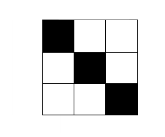
\includegraphics[width=0.5\textwidth]{Screenshot_2025_0821_162234.png}
\caption{}                                     
\label{fig:Q3}                             
\end{figure}

\begin{multicols}{4}
\begin{enumerate}
    \item 2
    \item 9
    \item 3
    \item 6
\end{enumerate}
\end{multicols}

\item There are 4 red, 5 green, and 6 blue balls inside a box. If $N$ number of balls are picked simultaneously, what is the smallest value of $N$ that guarantees there will be at least two balls of the same colour?  

One cannot see the colour of the balls until they are picked.  

\hfill(GATE MN 2023)

\begin{multicols}{4}
\begin{enumerate}
    \item 4
    \item 15
    \item 5
    \item 2
\end{enumerate}
\end{multicols}
\item Consider a circle with its centre at the origin O(0,0), as shown. Two operations are allowed on the circle:  

Operation 1: Rotation in anti-clockwise direction by any angle.  
Operation 2: Reflection with respect to any line through the origin.  

Which one of the following shapes can be achieved through a combination of these two operations on the circle?  
\begin{figure}[H]
    \centering
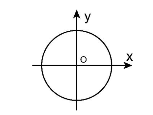
\includegraphics[width=0.6\textwidth]{Screenshot_2025_0822_110011.png}
\caption{}
    \label{fig:Q5}
\end{figure}


\hfill(GATE MN 2023)
\begin{multicols}{2}
	
	\begin{figure}[H]
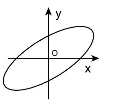
\includegraphics[width=0.45\textwidth]{Screenshot_2025_0822_110218.png} \\
		\caption*{(a)}
\label{fig:Q5option1}
 \end{figure}

\begin{figure}[H]
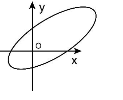
\includegraphics[width=0.45\textwidth]{Screenshot_2025_0822_110239.png} \\
	\caption*{(b)}
  \label{fig:Q5option2}
  \end{figure}

\begin{figure}[H]
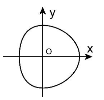
\includegraphics[width=0.45\textwidth]{Screenshot_2025_0822_110301.png} \\
	\caption*{(c)}
  \label{fig:Q5option3}
  \end{figure}

\begin{figure}[H]
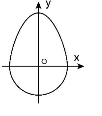
\includegraphics[width=0.45\textwidth]{Screenshot_2025_0822_110326.png} \\
	\caption*{(d)}
\label{fig:5option4}
 \end{figure}
\end{multicols}
\item Democracy is a system that provides equality and freedom. Two opinions about democracy are given below:  

(I) In democracy, one always respects one’s free choice to live, dress or eat in one’s own way.  
(II) In democracy, all citizens are free in matters of their dress, food and faith.  
(III) In democracy, sometimes one can suppress another person’s freedom of expression.  
(IV) In democracy, sometimes one expresses one’s free will by grilling a weaker person.  

Which of the above statements are consistent with the principles of democracy?  


\hfill(GATE MN 2023)
\begin{multicols}{2}
\begin{enumerate}
    \item (I) only  
    \item (II), (III) and (IV)  
    \item (I) and (II) only  
    \item (III) and (IV) only  
\end{enumerate}
\end{multicols}

\item Three hundred identical cubes are to be arranged in a straight line so that an identical number of cubes are placed on top of each cube (except the two at the ends). How many different arrangements are possible such that only 300 cubes are used?  


	\hfill(GATE MN 2023)
\begin{multicols}{4}
\begin{enumerate}
    \item 16  
    \item 48  
    \item 120  
    \item 720  
\end{enumerate}
\end{multicols}



\item Based only on the following passage, which one of the options can be inferred most accurately?  

\textit{When the emergency set up earlier, Appu’s mind lost its fresh joy, for he was no longer a carefree child. He was restless, agitated and had lost interest in his studies. Unable to resist the urge, Appu now stole a rupee from his mother’s box. For several days, Appu’s mind was in turmoil. He avoided his mother, for he was afraid that she might ask him for the missing rupee. When she didn’t, he felt relieved. Appu knew that his mother had discovered the theft, but she had chosen to remain silent. Appu’s sense of guilt increased day by day. Finally, unable to bear it any longer, he fell at his mother’s feet and cried. His mother lifted him gently, and wiping his tears, said: “Do not do it again, my son. Hereafter, you must become thoughtful.”}  



\hfill(GATE MN 2023)
\begin{enumerate}
    \item The mother was embarrassed about her daughter’s singing in a bus.  
    \item The mother’s feelings about her daughter’s singing in a bus was only of appreciation.  
    \item Therefore it was up to Appu to understand value of dignity from his father.  
    \item When Appu learned at home, his mother wanted him to become thoughtful.  

\end{enumerate}

    \item If $x$ satisfies the equation $4^{x^2} = 256$, then $x$ is equal to \underline{\hspace{2cm}}.
    

	    \hfill(GATE MN 2023)
    \begin{multicols}{4}
    \begin{enumerate}
        \item 1
        \item $\dfrac{1}{2}$
        \item $\log_{4} 8$
        \item $\log_{4} 3$
    \end{enumerate}
    \end{multicols}

    \item Consider a spheroidal globe rotating about an axis passing through its poles. There are three points $A, B, C$ situated respectively on the equator, the north pole and midway between the equator and the north pole on the meridian. Let $v_A, v_B, v_C$ and $r_A, r_B, r_C$ denote the tangential velocities and radial distances from the axis, respectively. 
    
    Which one of the following options is CORRECT?
    

    \hfill(GATE MN 2023)
    \begin{multicols}{2}
    \begin{enumerate}
        \item $v_A < v_C < v_B$
        \item $v_B < v_C < v_A$
        \item $v_C < v_B < v_A$
        \item $v_A < v_B < v_C$
    \end{enumerate}
    \end{multicols}
    

    \item The fault pattern shown in the figure is a case of \underline{\hspace{2cm}}.
    
    \begin{figure}[H]
    \centering
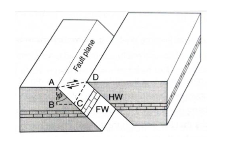
\includegraphics[width=0.5\textwidth]{Screenshot_2025_0822_112131.png}
\caption{}
    \label{fig:Q11}
\end{figure}
    

    \hfill(GATE MN 2023)
    \begin{multicols}{2}
    \begin{enumerate}
        \item Normal fault
        \item Reverse fault
        \item Strike slip fault
        \item Oblique slip fault
    \end{enumerate}
    \end{multicols}
    
 \item The joint pattern of a coal face shown in the figure represents \underline{\hspace{2cm}}.
    
    \begin{figure}[H]
    \centering
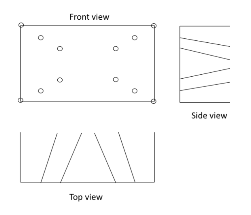
\includegraphics[width=0.6\textwidth]{Screenshot_2025_0822_112141.png}
\caption{}
    \label{fig:Q12}
\end{figure}


\hfill(GATE MN 2023)
    \begin{multicols}{2}
    \begin{enumerate}
        \item Burn cut
        \item Pyramid cut
        \item Wedge cut
        \item Drag cut
    \end{enumerate}
    \end{multicols}
   
\item A shear stress $\tau$ acts tangentially to the upper surface of a block and causes a small deformation as shown. The shear strain is calculated by


    \begin{figure}[H]
    \centering
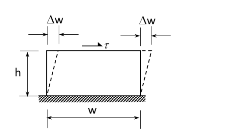
\includegraphics[width=0.6\textwidth]{Screenshot_2025_0822_113128.png}
\caption{}
    \label{fig:Q13}
\end{figure}


\hfill(GATE MN 2023)
\begin{multicols}{4}
\begin{enumerate}
    \item $\dfrac{\Delta x}{h}$  
    \item $\dfrac{\Delta x}{l}$  
    \item $\dfrac{2\Delta x}{h}$  
    \item $\dfrac{2\Delta x}{l}$  
\end{enumerate}
\end{multicols}

\item Given two vectors $A = 3\hat{i} + 2\hat{j}$ and $B = \hat{i} + \hat{j}$, the magnitude of projection of $A$ along $B$ is


	\hfill(GATE MN 2023)
\begin{multicols}{4}
\begin{enumerate}
    \item $\dfrac{5}{\sqrt{2}}$  
    \item $\dfrac{5}{\sqrt{3}}$  
    \item $\dfrac{3}{\sqrt{2}}$  
    \item $\dfrac{2}{\sqrt{3}}$  
\end{enumerate}
\end{multicols}
\item Axial stress versus axial strain curves for two test results of a porous rock from triaxial compression tests are shown in the figure.  
The pore water pressure for the curve B can be best explained by


    \begin{figure}[H]
    \centering
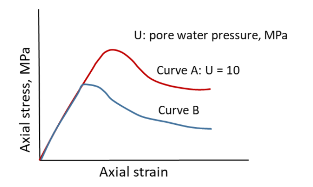
\includegraphics[width=0.6\textwidth]{Screenshot_2025_0822_113146.png}
\caption{}
    \label{fig:Q15}
\end{figure}


\hfill(GATE MN 2023)
\begin{multicols}{2}
\begin{enumerate}
    \item $U < 0$  
    \item $U = 0$  
    \item $U > 10$  
    \item $0 < U < 10$  
\end{enumerate}
\end{multicols}

\item Given two random variables $X$ and $Y$, the expected value $E(XY - 5Y)$ is


	\hfill(GATE MN 2023)
\begin{multicols}{4}
\begin{enumerate}
    \item $E(XY) - 5E(Y)$  
    \item $E(XY) - 5$  
    \item $5E(XY) - 5E(Y)$  
    \item $E(XY) - E(X)$  
\end{enumerate}
\end{multicols}

\item The reaction products of calcium hydroxide with acidic ferruginous mine water are


	\hfill(GATE MN 2023)
\begin{multicols}{2}
\begin{enumerate}
    \item FeO, Ca$^{2+}$ and H$_2$  
    \item Fe$_2$O$_3$, CaO and H$_2$O  
    \item Fe(OH)$_3$, Ca$^{2+}$ and OH$^-$  
    \item Fe$_2$(SO$_4$)$_3$, Ca$^{2+}$ and H$_2$O  
\end{enumerate}
\end{multicols}

\item An underground coal mine experienced 5 serious injuries, 15 reportable injuries, and 25 minor injuries during 2000.  
If the average employment in the mine is 1200, the total injury rate per 1000 persons is approximately


\hfill(GATE MN 2023)
\begin{multicols}{4}
\begin{enumerate}
    \item 51.0  
    \item 62.5  
    \item 37.5  
    \item 50.0  
\end{enumerate}
\end{multicols}

\item A linear programming problem is given as:  
\[
\text{Maximize } Z = 2x_1 + 3x_2
\]  
Subject to  
\[
2x_1 - x_2 \leq 20
\]  
\[
x_1 - 2x_2 \leq 20
\]  
\[
x_1, x_2 \geq 0
\]  
The problem has,  

\hfill(GATE MN 2023)
\begin{multicols}{2}
\begin{enumerate}
    \item Unbounded solution  
    \item Infeasible solution  
    \item Multiple optimal solutions  
    \item Unique optimal solution  
\end{enumerate}
\end{multicols}

\item A mother section (\(L=50\)m) makes two 2-m slice cuts for secondary blasting completely. What could be the immediate underground level rock cut and loading are mechanized? The suitable mining method is  


	\hfill(GATE MN 2023)
\begin{multicols}{2}
\begin{enumerate}
    \item Cut and fill stoping  
    \item Sub-level stoping  
    \item Unchecked open stoping  
    \item Breast stoping  
\end{enumerate}
\end{multicols}


\item \(x\) and \(y\) are functions of independent variables \(r\) and \(\theta\) given below:  
\[
x = r \cos \theta, \quad y = r \sin \theta
\]  
The Jacobian of \(x, y\) is  


\hfill(GATE MN 2023)
\begin{multicols}{2}
\begin{enumerate}
    \item \(\tan \theta\)  
    \item \(r \sin \theta \cos \theta\)  
    \item \(r^2\)  
    \item \(r\)  
\end{enumerate}
\end{multicols}


\item In project scheduling techniques, the CORRECT statement is  


	\hfill(GATE MN 2023)
\begin{multicols}{2}
\begin{enumerate}
    \item Both CPM and PERT are deterministic  
    \item Both CPM and PERT are probabilistic  
    \item CPM is deterministic and PERT is probabilistic  
    \item CPM is probabilistic and PERT is deterministic  
\end{enumerate}
\end{multicols}

\item As per DGMS guidelines, the risk score in Safety Management Plan for a hazard is computed as  


	\hfill(GATE MN 2023)
\begin{multicols}{2}
\begin{enumerate}
    \item Consequence × Exposure  
    \item Consequence × Exposure × Probability  
    \item Exposure × Probability  
    \item Consequence × Probability  
\end{enumerate}
\end{multicols}

\item Match the following items with their respective counters
\begin{table}[H]
    \centering\normalsize

\begin{tabular}{cc}

List-I & List-II \\
\hline
P. Isopleths & (1) Slope \\
Q. Isohyets  & (2) Rainfall \\
R. Isotachs  & (3) Wind velocity \\
S. Isochores & (4) Temperature \\

\end{tabular}
\caption{}                                          
\label{tab:Q24}                               
\end{table}


\hfill(GATE MN 2023)

\begin{multicols}{2}
\begin{enumerate}
    \item P--4, Q--2, R--3, S--1
    \item P--2, Q--3, R--1, S--4
    \item P--3, Q--2, R--1, S--4
    \item P--4, Q--1, R--2, S--3
\end{enumerate}
\end{multicols}


\item In an astronomical survey at a given station, the pole star is located at an angle of \(27^\circ\) from the horizon. The latitude of the survey station in degrees is  


	\hfill(GATE MN 2023)
\begin{multicols}{4}
\begin{enumerate}[label=(\Alph*)]
    \item \(27^\circ N\)  
    \item \(63^\circ N\)  
    \item \(27^\circ S\)  
    \item \(63^\circ S\)  
\end{enumerate}
\end{multicols}

\item The position tracking of a point by GPS is based on the technique of

	\hfill(GATE MN 2023)
\begin{multicols}{2}
\begin{enumerate}
    \item Graphical resection
    \item Analytical resection
    \item Triangulation
    \item Trilateration
\end{enumerate}
\end{multicols}

\item Matrix $A$ is negative definite. Which one of the following is NOT the correct statement about the matrix?

	\hfill(GATE MN 2023)
\begin{multicols}{2}
\begin{enumerate}
    \item It is symmetric
    \item Determinant of $A$ is always less than zero
    \item All the eigenvalues are less than zero
    \item Trace of $A$ is always less than zero
\end{enumerate}
\end{multicols}

\item The average ore grade of a copper deposit is 0.9\%. The recovery of the metal after processing, smelting and refining is 85\%. If the selling price of refined copper is Rs.~400/kg, the break-even cutoff grade (in \% Cu) is \underline{\hspace{2cm}}..  
\textit{[rounded off to 1 decimal place]}

\hfill(GATE MN 2023)
\item A slope stability radar shows that the position of a point $P$ in a mine dump shifts from $(200.6,\, 700.1,\, 60.0)$ to $(200.5,\, 700.1,\, 60.75)$ over a time of 2 h. The net displacement of the point $P$ (in m) is \underline{\hspace{2cm}}..  
\textit{[rounded off to 2 decimal places]}

\hfill(GATE MN 2023)
\item A Mohr-Coulomb failure envelope of a sandstone rock is given as
\[
\sigma_{1} = 30 + 3.5\sigma_{3}
\]
where $\sigma_{1}$ and $\sigma_{3}$, measured in MPa, are the major and minor principal stresses respectively.  
The angle of the failure plane with the $\sigma_{3}$ axis in degree is \underline{\hspace{2cm}}.  

\textit{[rounded off to 1 decimal place]}


\hfill(GATE MN 2023)
\item A punch hole of diameter $10 \, \text{mm}$ is to be made in a $5 \, \text{mm}$ thick rock plate as shown.  
If the yield strength of rock plate is $25 \, \text{MPa}$, the punch force $P$ required in kN is \underline{\hspace{2cm}}. 


    \begin{figure}[H]
    \centering
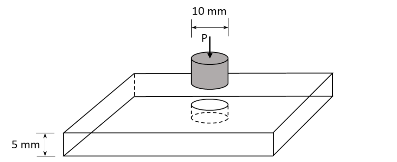
\includegraphics[width=0.6\textwidth]{Screenshot_2025_0822_121717.png}
\caption{}
    \label{fig:Q31}
\end{figure}



\textit{[rounded off to 1 decimal place]}   


\hfill(GATE MN 2023)
\item ``Critical subsidence'' has occurred on the surface due to mining of a flat longwall panel at a depth of 200 m. The width of the panel is 150 m. The maximum width of the panel in m that can be mined at a depth of 300 m to reach critical subsidence is \underline{\hspace{2cm}}..  
\textit{[rounded off to 1 decimal place]}


\hfill(GATE MN 2023)
\item To increase the resistance of a mine roadway by $1.5 \,\text{Ns}^2 \text{m}^{-8}$, the size (in m$^2$) of the regulator to be installed is \underline{\hspace{2cm}}..  
\textit{[rounded off to 2 decimal places]}


\hfill(GATE MN 2023)
\item A coal seam of 3.0 m height is mined with a double-ended ranging drum shearer (DERDS) for a web depth of 0.5 m. The coal density is 1.4 tonne/m$^3$. If the panel width is 150 m the production per cycle in tonne is \underline{\hspace{2cm}}..  
\textit{[rounded off to 2 decimal places]}


\hfill(GATE MN 2023)
\item In a panel with 50 workers, a miner typically consumes $2.5 \times 10^{-3}$ m$^3$/min of oxygen. The percentage of oxygen in the intake air is 20.9\%. To ensure minimum permissible oxygen requirement as per CMR 2017 the quantity of ventilating airflow (in m$^3$/min) to be supplied to the panel is \underline{\hspace{2cm}}..  
\textit{[rounded off to 2 decimal places]}


\hfill(GATE MN 2023)
\item In a quality control process of coal supplied to a thermal plant, the 3-sigma control limits for fixed carbon (FC) are defined by 40\% $\pm$ 15\%. The process is termed ``out of control'' if:  

\textbf{Rule 1:} 4 out of 5 successive values of FC are situated at the same side of the mean and at a distance more than 1 standard deviation.  

\textbf{Rule 2:} Any one value crosses any of the 3-sigma control limits.  

For the following continuous data of FC (\%): 49, 51, 56, 20, 46, 48, 47, 49, 45, 41, 42, 40, the process is  


\hfill(GATE MN 2023)
\begin{enumerate}
    \item out of control because of both rules 1 \& 2.
    \item out of control because of rule 1 only.
    \item out of control because of rule 2 only.
    \item not out of control.
\end{enumerate}

\item A tunnel of diameter 8 m is to be driven in a rock mass having quality index, Q of 1.0. Assume the excavation support ratio (ESR) of the tunnel is 1.0. The support requirement of the tunnel wall using fibre reinforced shotcrete (based on the chart prepared by Grimstad and Barton, 1993) is  

    \begin{figure}[H]
    \centering
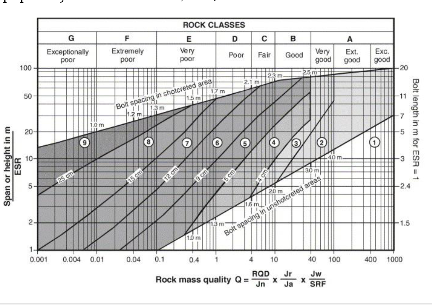
\includegraphics[width=0.6\textwidth]{Screenshot_2025_0822_122706.png}
\caption{}
    \label{fig:37}
\end{figure}


\hfill(GATE MN 2023)
\begin{enumerate}
    \item Shotcrete of thickness 9--12 cm, bolt length of 2.7--2.8 m
    \item Shotcrete of thickness 9--12 cm, bolt length of 3.0--3.2 m
    \item Shotcrete of thickness 5--9 cm, bolt length of 2.7--2.8 m
    \item Shotcrete of thickness 5--9 cm, bolt length of 2.5--2.6 m
\end{enumerate}

 
\item Match the following devices with their intended applications.  
\begin{table}[H]                                   
	\centering\normalsize
\begin{tabular}{|c|l|c|l|}
\hline
\textbf{Device} & & \textbf{Application} & \\
\hline
(P) & Ground Penetrating Radar & (1) & Spatial positioning of a point \\\hline
(Q) & Tactile Sensor           & (2) & Measurement of a borehole deviation \\\hline
(R) & Global Navigation Satellite System & (3) & Robotic Arm \\\hline
(S) & Digital Inclinometer     & (4) & Locating subsurface features \\
\hline
\end{tabular}
\caption{}                    
\label{tab:Q38}                  
\end{table}

\hfill(GATE MN 2023)
\begin{multicols}{2}
\begin{enumerate}[label=(\Alph*)]
    \item P=1 ; Q=2 ; R=3 ; S=4
    \item P=4 ; Q=3 ; R=1 ; S=2
    \item P=3 ; Q=4 ; R=2 ; S=1
    \item P=4 ; Q=3 ; R=2 ; S=1
\end{enumerate}
\end{multicols}

\item The evaluation of the integral  
\[
I = \int e^{x^e + x^e} \, dx
\]  
yields  


\hfill(GATE MN 2023)
\begin{multicols}{2}
\begin{enumerate}[label=(\Alph*)]
    \item $\ln(e^x + x^e)$
    \item $\dfrac{1}{e}\ln(e^x - x^e)$
    \item $\dfrac{1}{e}\ln(e^x + x^e)$
    \item $\ln(e^x - x^e)$
\end{enumerate}
\end{multicols}

\item Given the function  
\[
f(x) = |x| + |x-1|
\]  
For all the real values of $x$, which one of the following statements is CORRECT?


\hfill(GATE MN 2023)
\begin{enumerate}[label=(\Alph*)]
    \item The function is continuous and not differentiable at one point.
    \item The function is continuous but not differentiable at two points.
    \item The function is discontinuous.
    \item The function is continuous and differentiable.
\end{enumerate}

\item The slope and intercept values of three linear equations are  

	\begin{table}{H}
		\normalsize
\begin{tabular}{|c|c|c|}
\hline
\textbf{Equation no.} & \textbf{Slope} & \textbf{Intercept} \\
\hline
1 & 2.0 & 3.0 \\\hline
2 & 4.0 & 5.0 \\\hline
3 & 6.0 & 2.0 \\
\hline
\end{tabular}
		\caption{}
		\label{tab:Q41}
		\end{table}

The above system of equations has  


\hfill(GATE MN 2023)
\begin{multicols}{2}
\begin{enumerate}
    \item Trivial solution
    \item A single solution
    \item Multiple solutions
    \item No Solution
\end{enumerate}
\end{multicols}

\item A regression line is constructed between shovel production rate and shovel swing angle for 50 observations as shown below.  
\begin{table}[H]                                    
\centering\normalsize

\begin{tabular}{|c|c|c|}
\hline
 & Estimated parameter & Standard error \\
\hline
Intercept & 29.6 & 13.45 \\
Slope     & 2.5  & 1.32 \\
\hline
\end{tabular}
\caption{}                  
\label{tab:Q41}                  
\end{table}

t-values corresponding to level of significance (P) and degree of freedom (DF)


    \begin{figure}[H]
    \centering
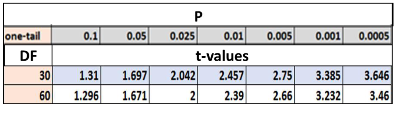
\includegraphics[width=0.6\textwidth]{Screenshot_2025_0822_125446.png}
\caption*{}
    \label{fig:Q42}
\end{figure}
If residuals are normally distributed and significance tests of the parameters are conducted at 0.05 significance level, the true statement is \underline{\hspace{2cm}}...  



\hfill(GATE MN 2023)
\begin{enumerate}
    \item Both intercept and slope are significant.
    \item Intercept is significant but slope is not significant.
    \item Intercept is not significant but slope is significant.
    \item Both intercept and slope are not significant.
\end{enumerate}



\item A duct of diameter 0.60 m with an exhausting fan has $-97.5$ mm wg static pressure behind the fan when the air flow rate is 4.0 m$^3$/s. If an evasee with inlet to outlet area ratio of 1:4 and efficiency 60\% is attached to the outlet of the fan, the static pressure of the fan in mm of wg becomes \underline{\hspace{2cm}}...  


	\hfill(GATE MN 2023)

\begin{multicols}{4}
\begin{enumerate}
    \item -104.26
    \item -99.13
    \item -90.73
    \item -80.6
\end{enumerate}
\end{multicols}
\item Coordinate of two points A and B are (E 0 m, N 200 m) and (E 300 m, N 200 m), respectively. The bearing of two lines AQ and BO are $67^\circ$ and $53^\circ$, respectively. The easting of point O, in m, is \underline{\hspace{2cm}}...  

\textit{[rounded off to 2 decimal places]}  


\hfill(GATE MN 2023)
\item Data related to a surface miner operation are given below:  

\begin{tabular}{ll}
Drum width (m) & : 3.0 \\
Average cutting depth (cm) & : 20 \\
Average cutting speed (m/min) & : 25 \\
Length of pit (m) & : 500 \\
Turning time (min) & : 2 \\
Truck exchange time (s) & : 30 \\
Truck capacity (m$^3$) & : 15 \\
\end{tabular}


Considering \textit{in situ} volume, the production rate of the surface miner in m$^3$/hr is \underline{\hspace{2cm}}...  

\textit{[rounded off to 1 decimal place]}  


\hfill(GATE MN 2023)

\item A continuous miner served by two shuttle cars produces 240 tonne/hr. The capacity of each shuttle car is 10 tonne. When a single shuttle car operates, the cycle time becomes 4 min. In case one of the shuttle cars is under break-down, the reduction in hourly production from that of two cars in percent is \underline{\hspace{2cm}}...  


	\hfill(GATE MN 2023)
\begin{multicols}{4}
\begin{enumerate}
    \item 25
    \item 33.33
    \item 40
    \item 50
\end{enumerate}
\end{multicols}


\item A circular tunnel is developed in a biaxial \textit{in situ} stress field as shown in the figure. 
If the ratio between tangential stress at the boundary point A and that at the boundary point B is $2.0$, the value of $k$ is \underline{\hspace{2cm}}.  

\textit{[rounded off to 2 decimal places]}  


    \begin{figure}[H]
    \centering
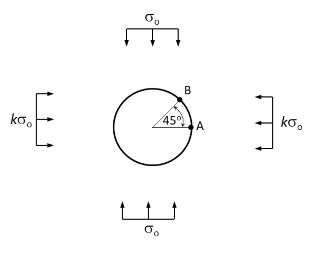
\includegraphics[width=0.6\textwidth]{Screenshot_2025_0822_130717.png}
\caption{}
    \label{fig:Q47}
    \end{figure}

\hfill(GATE MN 2023)

\item Strength of a rectangular coal pillar in MPa is given by  

\[
S_p = S_1 \left( 6.64 + 0.54 \frac{w}{h} - 0.18 \frac{w^2}{h} \right)
\]  

where $w \, (\geq w)$ and $h$ are width, length and height of the pillar, respectively. The parameter $S_1$ is constant.  

A 30 m square pillar is split into two halves as shown in the figure. The height of the pillar is 3 m. The ratio of safety factors between one half-pillar and the original square pillar is \underline{\hspace{2cm}}.  

\textit{[rounded off to 2 decimal places]}  


    \begin{figure}[H]
    \centering
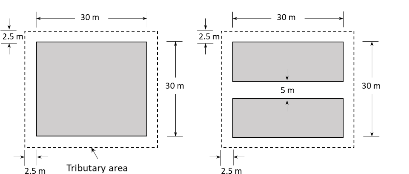
\includegraphics[width=0.6\textwidth]{Screenshot_2025_0822_130730.png}
\caption{}
    \label{fig:Q48}
\end{figure}


\hfill(GATE MN 2023)
\item A dozer pushes up a $100 \, \text{kg}$ spool of cable along a $20^\circ$ incline road at a constant velocity as shown in the figure.  
The coefficient of static friction between the dozer bucket and the spool (Point B) is $0.45$, and coefficient of kinetic friction between road and the spool (Point A) is $0.15$.  

Consider the spool only slides up the incline. The maximum normal force in N acting at Point B, is \underline{\hspace{2cm}}.  

\textit{[rounded off to 1 decimal place]}  


    \begin{figure}[H]
    \centering
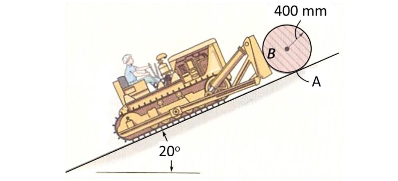
\includegraphics[width=0.6\textwidth]{Screenshot_2025_0822_130750.png}
\caption{}
    \label{fig:Q49}
\end{figure}


\hfill(GATE MN 2023)
\item Stress waves are sent from the transmitter A to the receiver B through an isotropic and elastic cylindrical rock specimen as shown in the figure.  

The length of the specimen is 100 mm. The travel time of longitudinal and shear waves are $0.025 \, \text{ms}$ and $0.04 \, \text{ms}$, respectively. The Poisson’s ratio of the rock specimen is \underline{\hspace{2cm}}.  

\textit{[rounded off to 2 decimal places]}  

    \begin{figure}[H]
    \centering
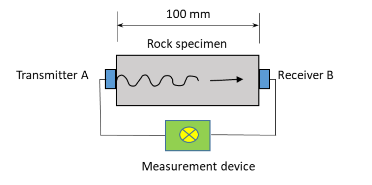
\includegraphics[width=0.6\textwidth]{Screenshot_2025_0822_131626.png}
\caption{}
    \label{fig:Q50}
\end{figure}


\hfill(GATE MN 2023)
\item A jointed rock sample is subjected to $20 \, \text{MPa}$ vertical stress as shown in the figure.  

The modulus of elasticity of the rock is $10 \, \text{GPa}$ and the normal stiffness of the joint surface is $5 \, \text{GPa/m}$. Assuming one-dimensional elastic behaviour of rock and joint, the displacement in mm of the loading surface AB is \underline{\hspace{2cm}}.  

\textit{[rounded off to 1 decimal place]}  

    \begin{figure}[H]
    \centering
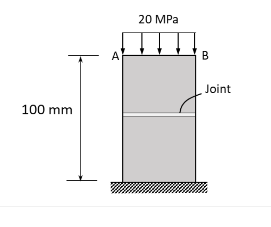
\includegraphics[width=0.6\textwidth]{Screenshot_2025_0822_131639.png}
\caption{}
    \label{fig:Q51}
\end{figure}


\hfill(GATE MN 2023)
\item An unmanned aerial vehicle (UAV) with payload of $2 \, \text{kg}$ reaches vertically $100 \, \text{m}$ in $10 \, \text{s}$ at uniform velocity. The self-weight of the UAV is $1.2 \, \text{kg}$. The power required in lifting in kW is \underline{\hspace{2cm}}.  

\textit{[rounded off to 2 decimal places]}  

\hfill(GATE MN 2023)

\item An irregular shaped rock sample of mass $60 \, \text{g}$ displaces $27 \, \text{g}$ of brine when submerged in a filled jar. The specific gravity of brine is $1.05$. The unit weight of the rock sample in $\text{kN/m}^3$ is \underline{\hspace{2cm}}.  

\textit{[rounded off to 2 decimal places]}  



\hfill(GATE MN 2023)
\item The reliability function of a pump is given as  

\[
R(t) = \exp\left[ - \left( \frac{t}{1000} \right)^{0.5} \right]
\]  

where $t$ stands for time in years. If the pump comes with a six-month warranty, the number of years for the pump to attain a reliability of 0.9 is \underline{\hspace{2cm}}.  

\textit{[rounded off to 2 decimal places]}  


\hfill(GATE MN 2023)
\item In a sample of groundwater, the concentration of Ca$^{2+}$ is $200 \,\text{mg/l}$.  
The corresponding calcium carbonate hardness in mg/l is \underline{\hspace{2cm}}.  

\textit{[rounded off to 1 decimal place]}  



\hfill(GATE MN 2023)
\item A thermal power station receives coal of calorific value $4000 \,\text{kcal/kg}$ and uses $7000$ tonnes of coal every day.  
Assuming $860 \,\text{kcal}$ is the heat equivalent of $1.0 \,\text{kWh}$, for a thermal efficiency of $40\%$ and electrical efficiency of $85\%$ the power generation per day in MWh is \underline{\hspace{2cm}}.  

\textit{[rounded off to 1 decimal place]}  



\hfill(GATE MN 2023)
\item A coal company has three mines which transport coal to four washeries.  
The daily production from each mine, the demand at each washery and unit transportation cost from each mine to each washery are given in table.  

\begin{table}[H]                                  
	\centering\normalsize
\begin{tabular}{|c|c|c|c|c|c|}
\hline
Mine & W1 & W2 & W3 & W4 & Supply (tonnes/day) \\
\hline
M1 & 40 & 50 & 90 & 100 & 900 \\\hline
M2 & 90 & 70 & 80 & 120 & 1800 \\\hline
M3 & 80 & 40 & 70 & 100 & 2000 \\
\hline
Demand (tonnes/day) & 400 & 1200 & 1500 & 1600 & \\
\hline
\end{tabular}
\caption{}                                   
\label{tab:Q57}                             
\end{table}

The cost of initial basic feasible solution using Vogel’s approximation method is \underline{\hspace{2cm}}.  

\textit{[rounded off to 1 decimal place]}  


\hfill(GATE MN 2023)
\item A workshop has four tasks and equal number of machines to perform the tasks.  
Each of the machines can perform only one of the four tasks. The estimated cost at each of the machines to complete each task is given in table:  


\begin{table}[H]
\centering\normalsize
\begin{tabular}{|c|c|c|c|c|}
\hline
\textbf{MACHINE} & \multicolumn{4}{c|}{\textbf{TASK}} \\ \hline
& T1 & T2 & T3 & T4 \\ \hline
M1 & 10 & 40 & 60 & 30 \\ \hline
M2 & 90 & 70 & 100 & 90 \\ \hline
M3 & 40 & 50 & 110 & 70 \\ \hline
M4 & 80 & 70 & 80 & 50 \\ \hline
\end{tabular}
	\caption{}
	\label{tab:Q58}
\end{table}



The total cost of optimal assignment is \underline{\hspace{2cm}}.  

\textit{[rounded off to 1 decimal place]}  



\hfill(GATE MN 2023)
\item The time between consecutive accidents in days in an underground coal mine in a year are as follows:  

10, 15, 6, 18, 12, 14, 16, 9, 21, 15, 26, 18, 22, 25, 13  

Assuming exponential distribution, the probability that there will be no accident over a 10-day period is \underline{\hspace{2cm}}.  

\textit{[rounded off to 2 decimal places]}  



\hfill(GATE MN 2023)
\item A surface mine blast pattern has spacing $4 \, \text{m}$ and burden $3 \, \text{m}$.  
The diameter of the drill hole is $110 \, \text{mm}$. The drilling length is $8.8 \, \text{m}$ including subgrade of $10\%$.  
The bulk explosive density is $900 \,\text{kg/m}^3$.  

If the powder factor is $2.5 \,\text{m}^3/\text{kg}$, the charge length in m is \underline{\hspace{2cm}}.  

\textit{[rounded off to 2 decimal places]}  


\hfill(GATE MN 2023)
\item A mining company makes an initial investment of Rs 200 crore on a project.  

    \begin{figure}[H]
    \centering
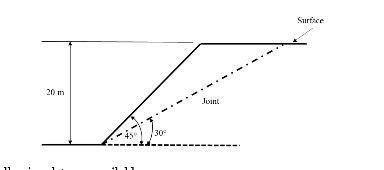
\includegraphics[width=0.6\textwidth]{Screenshot_2025_0822_133458.png}
\caption{}
    \label{fig:Q61}
\end{figure}
The following data are available:  
\begin{enumerate}
    \item Production life : 3 years  
    \item Year wise production after gestation period (Mtonne) : 1.0, 2.0, and 1.0  
    \item Stripping ratio : 1.5 m$^3$/tonne  
    \item Selling price of ore : Rs.\ 2000 per tonne  
    \item Ore mining cost : Rs.\ 500 per tonne  
    \item Waste mining cost : Rs.\ 500 per m$^3$  
    \item Discount rate : 10\%  
\end{enumerate}

By ignoring any other cash-flows, if the NPV of the project becomes Rs.\ 5.367 crore, the gestation period of the project, in years, is \underline{\hspace{2cm}}.  

\textit{[rounded off to the nearest integer]}  



\hfill(GATE MN 2023)
\item A rock slope is intercepted by a joint plane at an angle $30^\circ$ as shown in figure.  

The following data are available:  
\begin{enumerate}
    \item Unit weight of the rock : 20 kN/m$^3$  
    \item Cohesion of joint : 30 kPa  
    \item Friction angle of joint : $22^\circ$  
\end{enumerate}

The factor of safety of the rock slope to slide along the joint plane is \underline{\hspace{2cm}}.  

\textit{[rounded off to 2 decimal places]}  

\hfill(GATE MN 2023)


\item A mine void of width 20 m, length 50 m and height 30 m is to be filled with mill tailings based cemented paste backfill (CPB).  

The CPB contains tailings:cement:water as 1.0:0.1:0.2 by weight. The specific gravity of tailings and cement are 2.8 and 2.4 respectively. Assuming 20\% of the original volume of water is retained in the final backfill, the amount of cement in tonne required so as to fill the void completely is \underline{\hspace{2cm}}.  

\textit{[rounded off to nearest integer]}  


\hfill(GATE MN 2023)

\item A fan installed in a mine ventilation system circulates 30 m$^3$/s of air to two districts A and B as shown in figure below.  

It is desired to increase the quantity of air by 20\% in the district B using a booster fan in it. Assuming that the main fan pressure is unchanged, the pressure of the booster fan, in Pa, is \underline{\hspace{2cm}}.  


    \begin{figure}[H]
    \centering
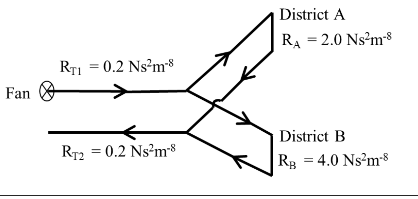
\includegraphics[width=0.6\textwidth]{Screenshot_2025_0822_133511.png}
\caption{}
    \label{fig:Q64}
\end{figure}

\textit{[rounded off to 2 decimal places]}  


\hfill(GATE MN 2023)
\item Data related to a water turbine pump with backward bladed impellers are given below:

    \begin{enumerate}
        \item Impeller diameter : 35 cm
        \item RPM : 1200
        \item Angle of curvature of blade : $30^\circ$
        \item Radial velocity of discharge : 2 m/s
        \item Manometric efficiency : 0.8
    \end{enumerate}

The number of impellers required in the pump to lift water by a height 300 m is \underline{\hspace{2cm}}.  

\textit{[rounded off to higher integer]}  



\hfill(GATE MN 2023)

\end{enumerate}
\begin{center}
	\huge{END OF QUESTION PAPER}
\end{center}
\end{document}

